%!TEX root = Tesi__Simone_Mariotti.tex
\chapter{Componenti del robot}
\fancyhead[R]{\bfseries Componenti del robot} 	 	
\fancyfoot[C]{\thepage } 
\section{Hardware}
\subsection{UDOO Quad}
UDOO è un progetto tutto italiano di una piattaforma hardware destinata alla 
generazione dei ``makers'', cioè quelle persone che vogliono realizzare i 
proprie progetti con le tecnologia a basso costo ad oggi disponibili. La 
scheda ha visto la luce dopo una sorprendente campagna di crowdfunding
\footnote{dall'inglese crowd, folla e funding, finanziamento. In italiano finanziamento collettivo.} terminata l'8 Giugno 2013 con 4172 donazioni per un totale di \$641.612 a fronte di \$27.000 richiesti per iniziare la produzione. Per permettere l'utilizzo di librerie e applicazioni computazionalmente pesanti 
come openCV, PureData e altre UDOO monta un processore ARM Freescale i.MX6 
Cortex-A9 Quad core 1GHz che supporta sia Android che Linux. Il tutto è 
completato da una GPU Vivante, 1GB di RAM DDR3, numerose porte di I/O come 
SATA, microfono, audio out, Ethernet, HDMI, USB, connettore per display LVDS 
con touch screen, connettore CSI per camera esterna e connettività bluetooth e 
Wi-Fi. La periferica di ``boot'' è una microSD il che permette un rapido 
passaggio da Linux a Android e viceversa. Quello che però rende veramente 
unica questa piattaforma, e che ne ha fatto la nostra scelta per questo 
progetto di tesi, è la presenza di un Arduino DUE completamente integrato 
nella stessa board. 
E' presente una CPU Atmel SAM3X8E ARM Cortex-M3 \footnote{la stessa di cui 
dispone l'Arduino DUE} e 76 GPIO\footnote{General Purpose Input/Output}, di 
cui 62 digitali e 14 digitali/analogici, disposti per essere perfettamente 
compatibili con la piedinatura dell'Arduino DUE e dell'Arduino UNO Rev.3.

\begin{figure}[!htb] \center
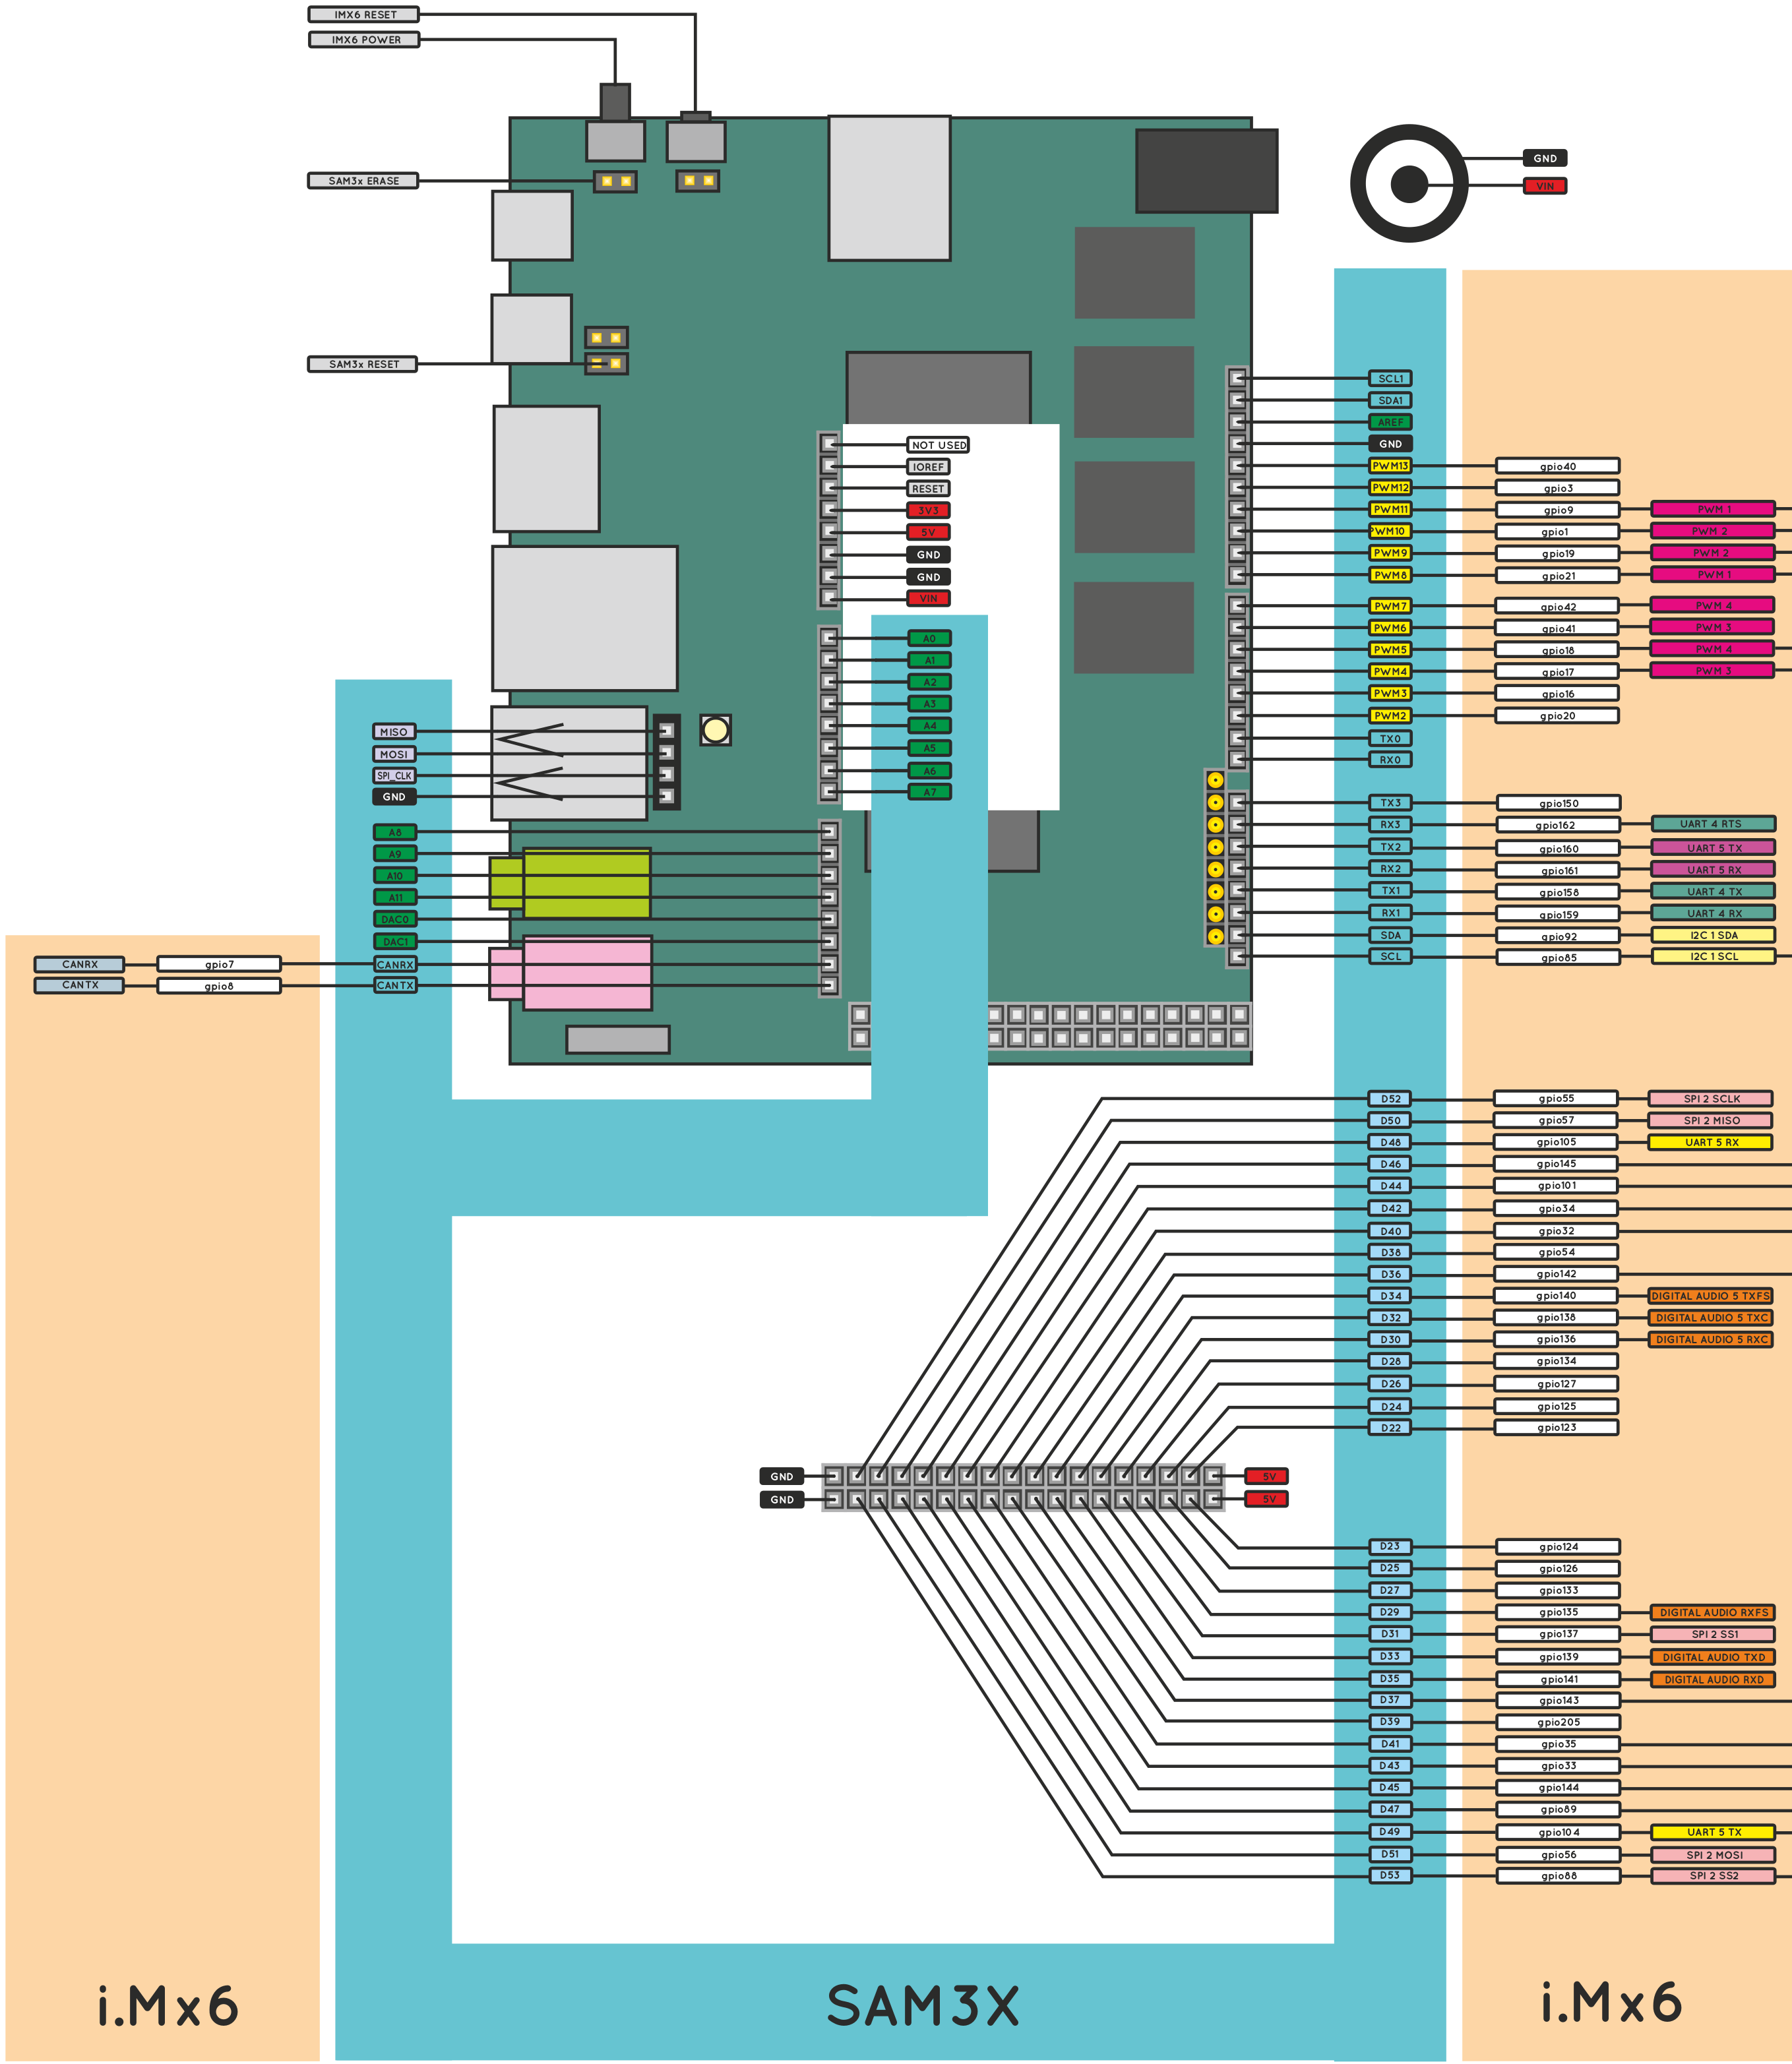
\includegraphics[width=\textwidth]{immagini/udoo_pinout.png}
\caption{Schema piedinatura UDOO} 
\end{figure}

La presenza di un Arduino DUE all'interno della board rende UDOO una scheda di 
prototipazione a tutti gli effetti e apre nuovi interessanti scenari e 
possibilità unendo la versatilità e semplicità di Arduino, la potenza di 
calcolo del Freescale i.MX6 e le numerose periferiche disponibili per Linux o 
Android.\\
Essendo una piattaforma open-source è possibile accedere alla shell del 
sistema operativo come root tramite la porta seriale integrata e modificare a 
piacimento la configurazione del sistema operativo. Arduino è collegato al 
Freescale i.MX6 tramite un bus interno e quindi viene rilevato come una 
normale periferica USB da Linux; su Android la comunicazione tra i due 
dispositivi avviene sullo stesso bus ma usa lo standard USB OTG\footnote{On-The
-Go è una specifica che permettere di agire come host ad un qualsiasi  
dispositivo (tipicamente smartphone e tablet). A differenza dell'USB classico 
l'OTG è driver-less, cioè non necessita l'installazione di driver specifici 
per ogni dispositivo}. L'interconnessione tra l'accessorio Arduino e 
l'applicazione Android è realizzata tramite l'ADK\footnote{Android Development 
Kit} 2012, di cui parleremo più avanti in questo stesso capitolo, che permette 
l'integrazione delle più disparate periferiche a dispositivi Android tramite 
una connessione USB o Bluetooth.
\subsection {Tank Kit}
Per dare la giusta stabilità e manovrabilità al robot si è deciso di usare una
 locomozione a cingoli che richiede solo due motori e permette di ruotare sul 
 posto o comunque in spazi ristretti: la nostra scelta è stata il ``Multi-
 Chassis - Tank Version''. Questa piattaforma, appositamente pensata per la 
 realizzazione di robot multifunzione, si è rivelata la scelta perfetta in 
 quanto possiede due potenti motori DC già forniti di riduttori 48:1 per 
 affrontare terreni impervi e scoscesi, quattro ruote da 52 mm di diametro a 
 cui sono applicati i due cingoli. E' presente anche un alloggiamento per un 
 servomotore standard che nella nostra applicazione non è stato usato. 
 L'intelaiatura, di alluminio spesso 2,5 mm, presenta numerosi fori e asole
  per il montaggio di accessorie quali sensori, staffe e motori. Presenta
  inoltre un ``doppio fondo'' in cui sono alloggiati i motori DC e i riduttori 
  e in cui è possibile sistemare altri componenti che non debbano essere 
  facilmente accessibili.
\subsection {Sensori}
\subsubsection{Sensore di riflessività - QRD1114}
Avevamo la necessità di fornire al robot un modo per rilevare eventuali 
sconfinamenti dall'ambiente di test che fosse il più flessibile possibile. 
Abbiamo optato per il sensore di riflessività QRD1114 prodotto dalla Fairchild 
Semiconductor: questo sensore è costituito da un LED infrarosso e un 
fototransistor tarato sulla luce infrarossa e con filtro per la luce solare 
onde evitare disturbi. Il robot era stato pensato per lavorare su un tavolo o 
altra superficie con spigoli netti: per rilevare l'imminente caduta in questo 
tipo di ambiente sarebbe stato sufficiente un sensore di distanza puntato 
verso terra. Con il sensore di riflessività abbiamo reso possibile l'utilizzo 
in terra o comunque in ambienti estesi delimitati da un recinto spesso circa 
10cm realizzato con materiale a basse riflettività come del semplice 
cartoncino nero opaco. Il sensore non fa differenza tra il cartoncino nero o 
lo spazio a fianco di un tavolo, rileva semplicemente una riflessività vicina 
allo zero. Il sensore così come fornito dal produttore non è direttamente 
utilizzabile, per far si che Arduino potesse acquisire dal sensore valori 
proporzionali alla riflessività del materiale in esame abbiamo dovuto 
realizzare un circuito elettronico di interfaccia. 
\begin{figure}[!htb] \center
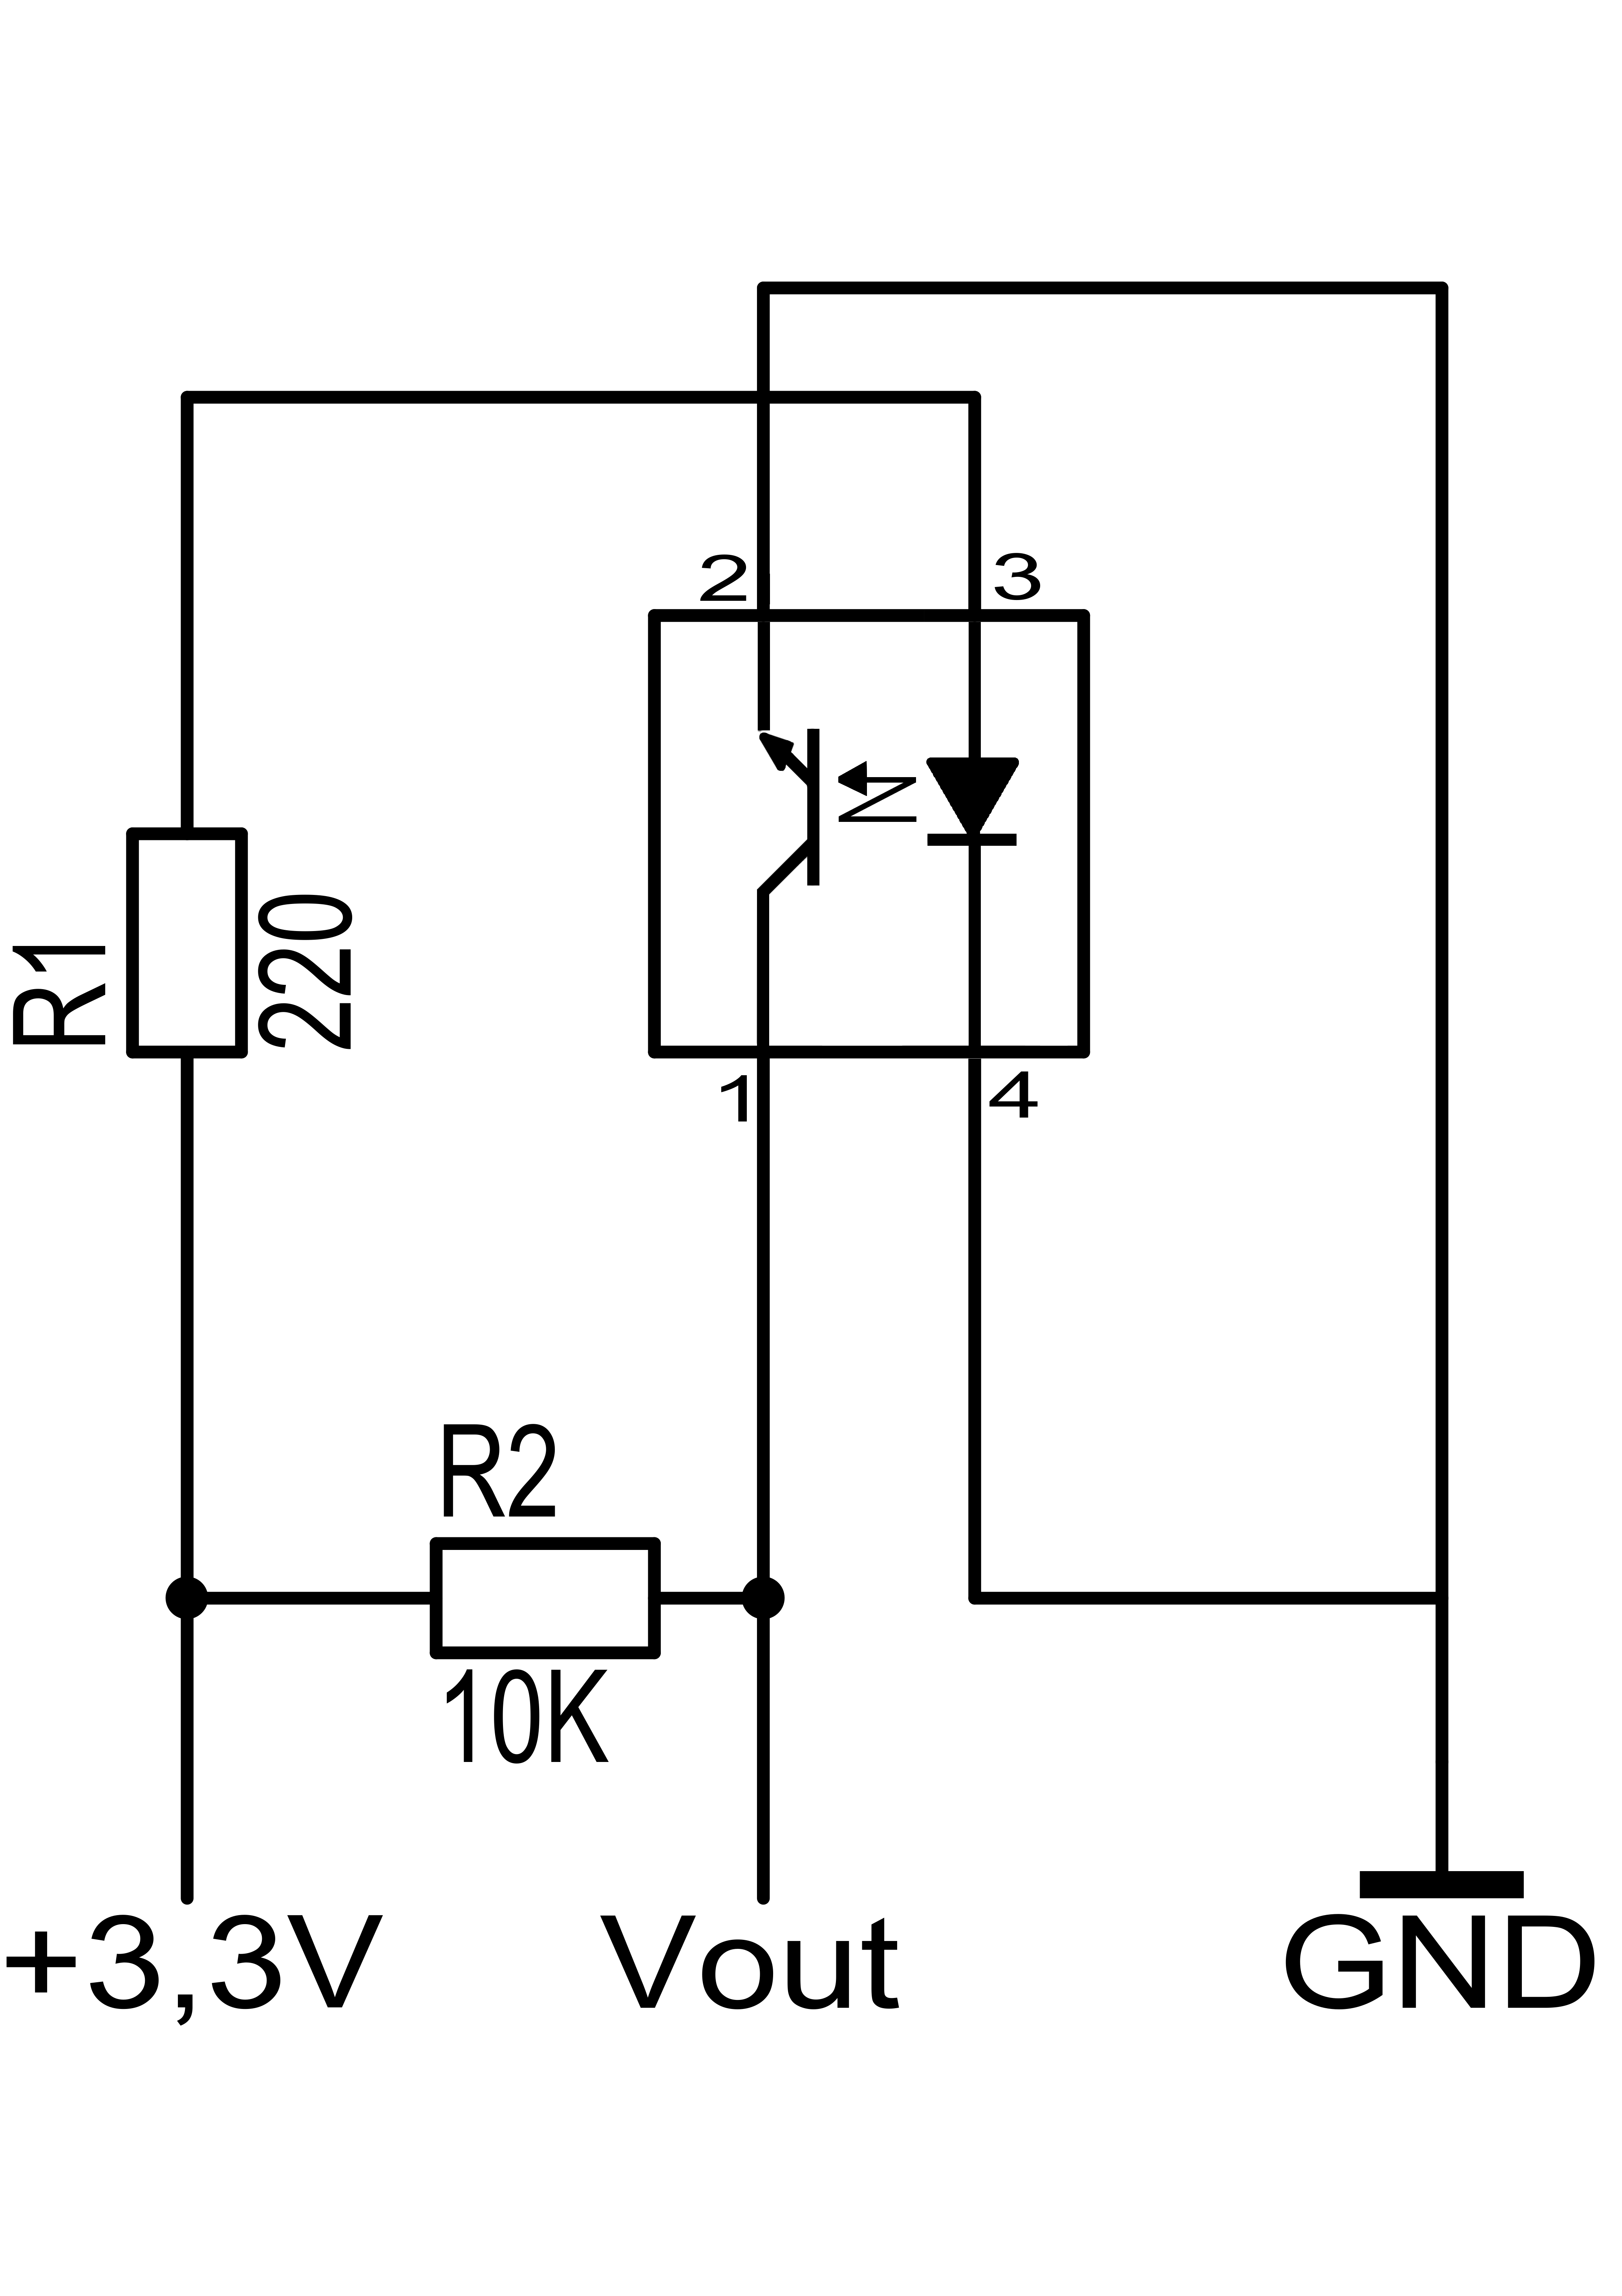
\includegraphics[scale=0.3]{immagini/QRD1114_Circuito.png}
\caption{Circuito di interfaccia tra Arduino DUE e il sensore QRD1114} 
\end{figure}
\\Il circuito alimenta il LED tramite una resistenza da 220$\Omega$ (\textit{R1}) 
e collega $V_{CC}$\footnote{pari a 3,3 $V$ nell'Arduino DUE} al collettore del 
fototransistor tramite una resistenza da 10 $k\Omega$ (\textit{R2}) mentre 
l'emettitore è collegato a terra; il punto da cui prelevare il segnale ($V_{OUT
}$) è tra \textit{R2} e il collettore. Il principio alla base del circuito è 
semplice: il LED è sempre acceso e illumina in modo diffuso parallelamente al 
fototransistor. Il fototransistor in assenza di luce o, nel nostro caso, in 
presenza di una bassa riflessività si trova in stato di interdizione; i pin di 
Arduino impostati come input sono in configurazione ``alta impedenza'', 
equivalenti ad un interruttore aperto dal punto di vista circuitale, quindi 
non c'è passaggio di corrente né tramite il transistor né tramite la 
resistenza \textit{R2} il che porta esattamente il valore di $V_{CC}$ in 
ingresso ad Arduino. Quando il fototransistor è totalmente illuminato, cioè in 
presenza di alta riflessività, entra in stato di conduzione così che nel punto 
$V_{OUT}$ si venga a trovare la massa. Ogni stato intermedio di illuminazione 
equivale ad una conduzione parziale del fotoresistore a cui corrisponde una 
tensione proporzionale alla riflessività sul pin $V_{OUT}$. Il sensore può 
essere utilizzato in modalità digitale o analogica semplicemente collegando il 
pin $V_{OUT}$ ad un pin digitale o analogico e cambiando la configurazione 
relativa all'interno della programmazione di Arduino. La configurazione 
digitale si è rivelata inadatta all'applicazione in quanto l'intervallo di 
valori che rappresenta un oggetto riflette nelle immediate vicinanze del 
sensore, e quindi lo stato di normale funzionamento, è troppo stretto e anche 
un minimo sussulto manda il robot in allarme sconfinamento. La configurazione 
analogica invece ci permette di avere circa 1024 valori discreti dal 
trasduttore, abbiamo quindi impostato una soglia oltre la quale il robot va in 
allarme sconfinamento; è importante notare che questa libertà nello scegliere 
una soglia di allarme ci permette di effettuare una calibrazione affinata in 
base al materiale su cui si svolge il test per minimizzare la possibilità di 
falsi positivi. 
\subsubsection{Sensore di distanza a ultrasuoni - HC-SR04}
Il robot aveva bisogno di conoscere la distanza degli oggetti che si trovavano 
di fronte ad esso, la scelta è ricaduta un sensore ad ultrasuoni, a discapito di
 uno ad infrarossi, per la totale assenza di disturbi dovuti all'illuminazione 
 dell'ambiente di test. In particolare abbiamo scelto il sensore HC-SR04 che 
 offre ottime prestazioni, è facile da integrare ed è di dimensioni contenute.\\
Il sensore può rilevare oggetti distanti da 2 cm a 400 cm con una risoluzione 
di 0,3 cm entro un cono frontale con apertura di 60$^\circ$, 30$^\circ$ per lato 
rispetto alla perpendicolare dal sensore.
\begin{figure}[!htb] \center
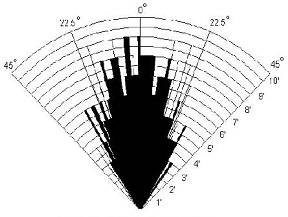
\includegraphics[scale=0.6]{immagini/HC-SR04_Angle.png}
\caption{Risposta del sensore rispetto alla posizione dell'ostacolo} 
\end{figure}
\\Il collegamento alla piattaforma di sviluppo è effettuato tramite quattro pin: 
\textit{$+5V$}, \textit{trig}, \textit{echo} e \textit{GND}.
Il funzionamento è piuttosto semplice, una volta alimentato il sensore si invia 
sul pin \textit{trig} un impulso di durata $10 \mu$s, il sensore invia 
quindi un impulso ultrasonico e restituisce sul pin \textit{echo} un segnale 
positivo di durata pari al tempo di percorrenza andata e ritorno del segnale 
ultrasonico. Una volta ottenuto il tempo di percorrenza si utilizza la formula 
del moto rettilineo uniforme:
$$v = \frac{\Delta s}{\Delta t}$$
sapendo che la velocità del suono a 20 $^\circ$C è approssimabile a 344 m/s allora 
la durata dell'impulso di $echo$ sarà compreso tra 116.3 $\mu$s e 23,26 ms 
rispettivamente per distanze percorse di 4 cm (2+2) e di 8 m (4+4).
\\Per ricavare la distanza ($d$) in centimetri a partire dalla durata dell'impulso 
notando che 344 m/s = 29,1 cm/$\mu$s e indicando con $T_e$ la durata dell'impulso 
di echo usiamo:
$$d=\frac{T_e}{2\cdot29,1}$$
Per quanto riguarda il collegamento ad Arduino se la nostra scheda accettasse 
input a 5 V questo sensore non avrebbe bisogno di nessun accorgimento per essere
 collegato, purtroppo però, anche se la nostra UDOO 
e l'Arduino DUE in essa integrato possono fornire alimentazione a 5 V, non possono 
accettare input allo stesso voltaggio ma solo a 3,3 V. 
\\Allo stesso modo del sensore QRD1114 ci serve un circuito di interfaccia che 
in questo caso sarà un semplice partitore di tensione il cui schema generico è 
riportato di seguito

\begin{figure}[!htb] \center
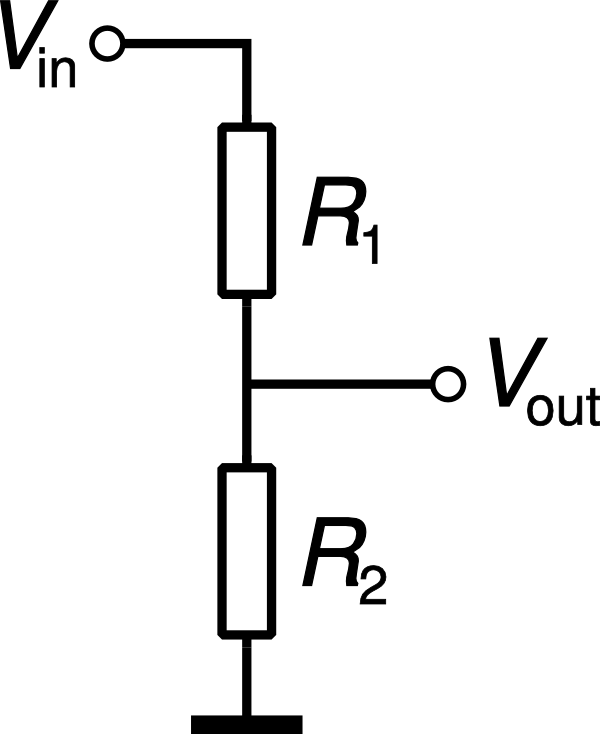
\includegraphics[scale=0.6]{immagini/Voltage_divider.png}
\caption{Schema generico del partitore di tensione} 
\end{figure}

Il partitore di tensione, a fronte di un noto valore di tensione di ingresso 
$V_{IN}$ riesce a fornirci il valore di tensione desiderato in uscita $V_{OUT}$ 
tramite due resistenze opportunamente dimensionate. 

La formula che regola il partitore di tensione è la seguente
$$V_{OUT}=V_{IN}\cdot\frac{R_2}{R_1+R_2}$$
nel nostro caso $V_{IN}$ = 5 V e $V_{OUT}$ = 3,3 V quindi scegliendo arbitrariamente 
il valore di $R_1$ 1 k$\Omega$ ricaviamo semplicemente il valore di $R_2$ tramite 
la formula inversa $$R_2 = R_1\cdot\frac{V_{OUT}}{V_{IN}-V_{OUT}}$$
che da come risultato 1941,48 $\Omega$; approssimando il valore appena calcolato
al più vicino taglio standard di resistenze, cioè $R_2 $ = 2 k$\Omega$, si ottiene $V_{OUT}$
 = $3,\overline{3}$ che è assolutamente accettabile.

\begin{figure}[H] \center
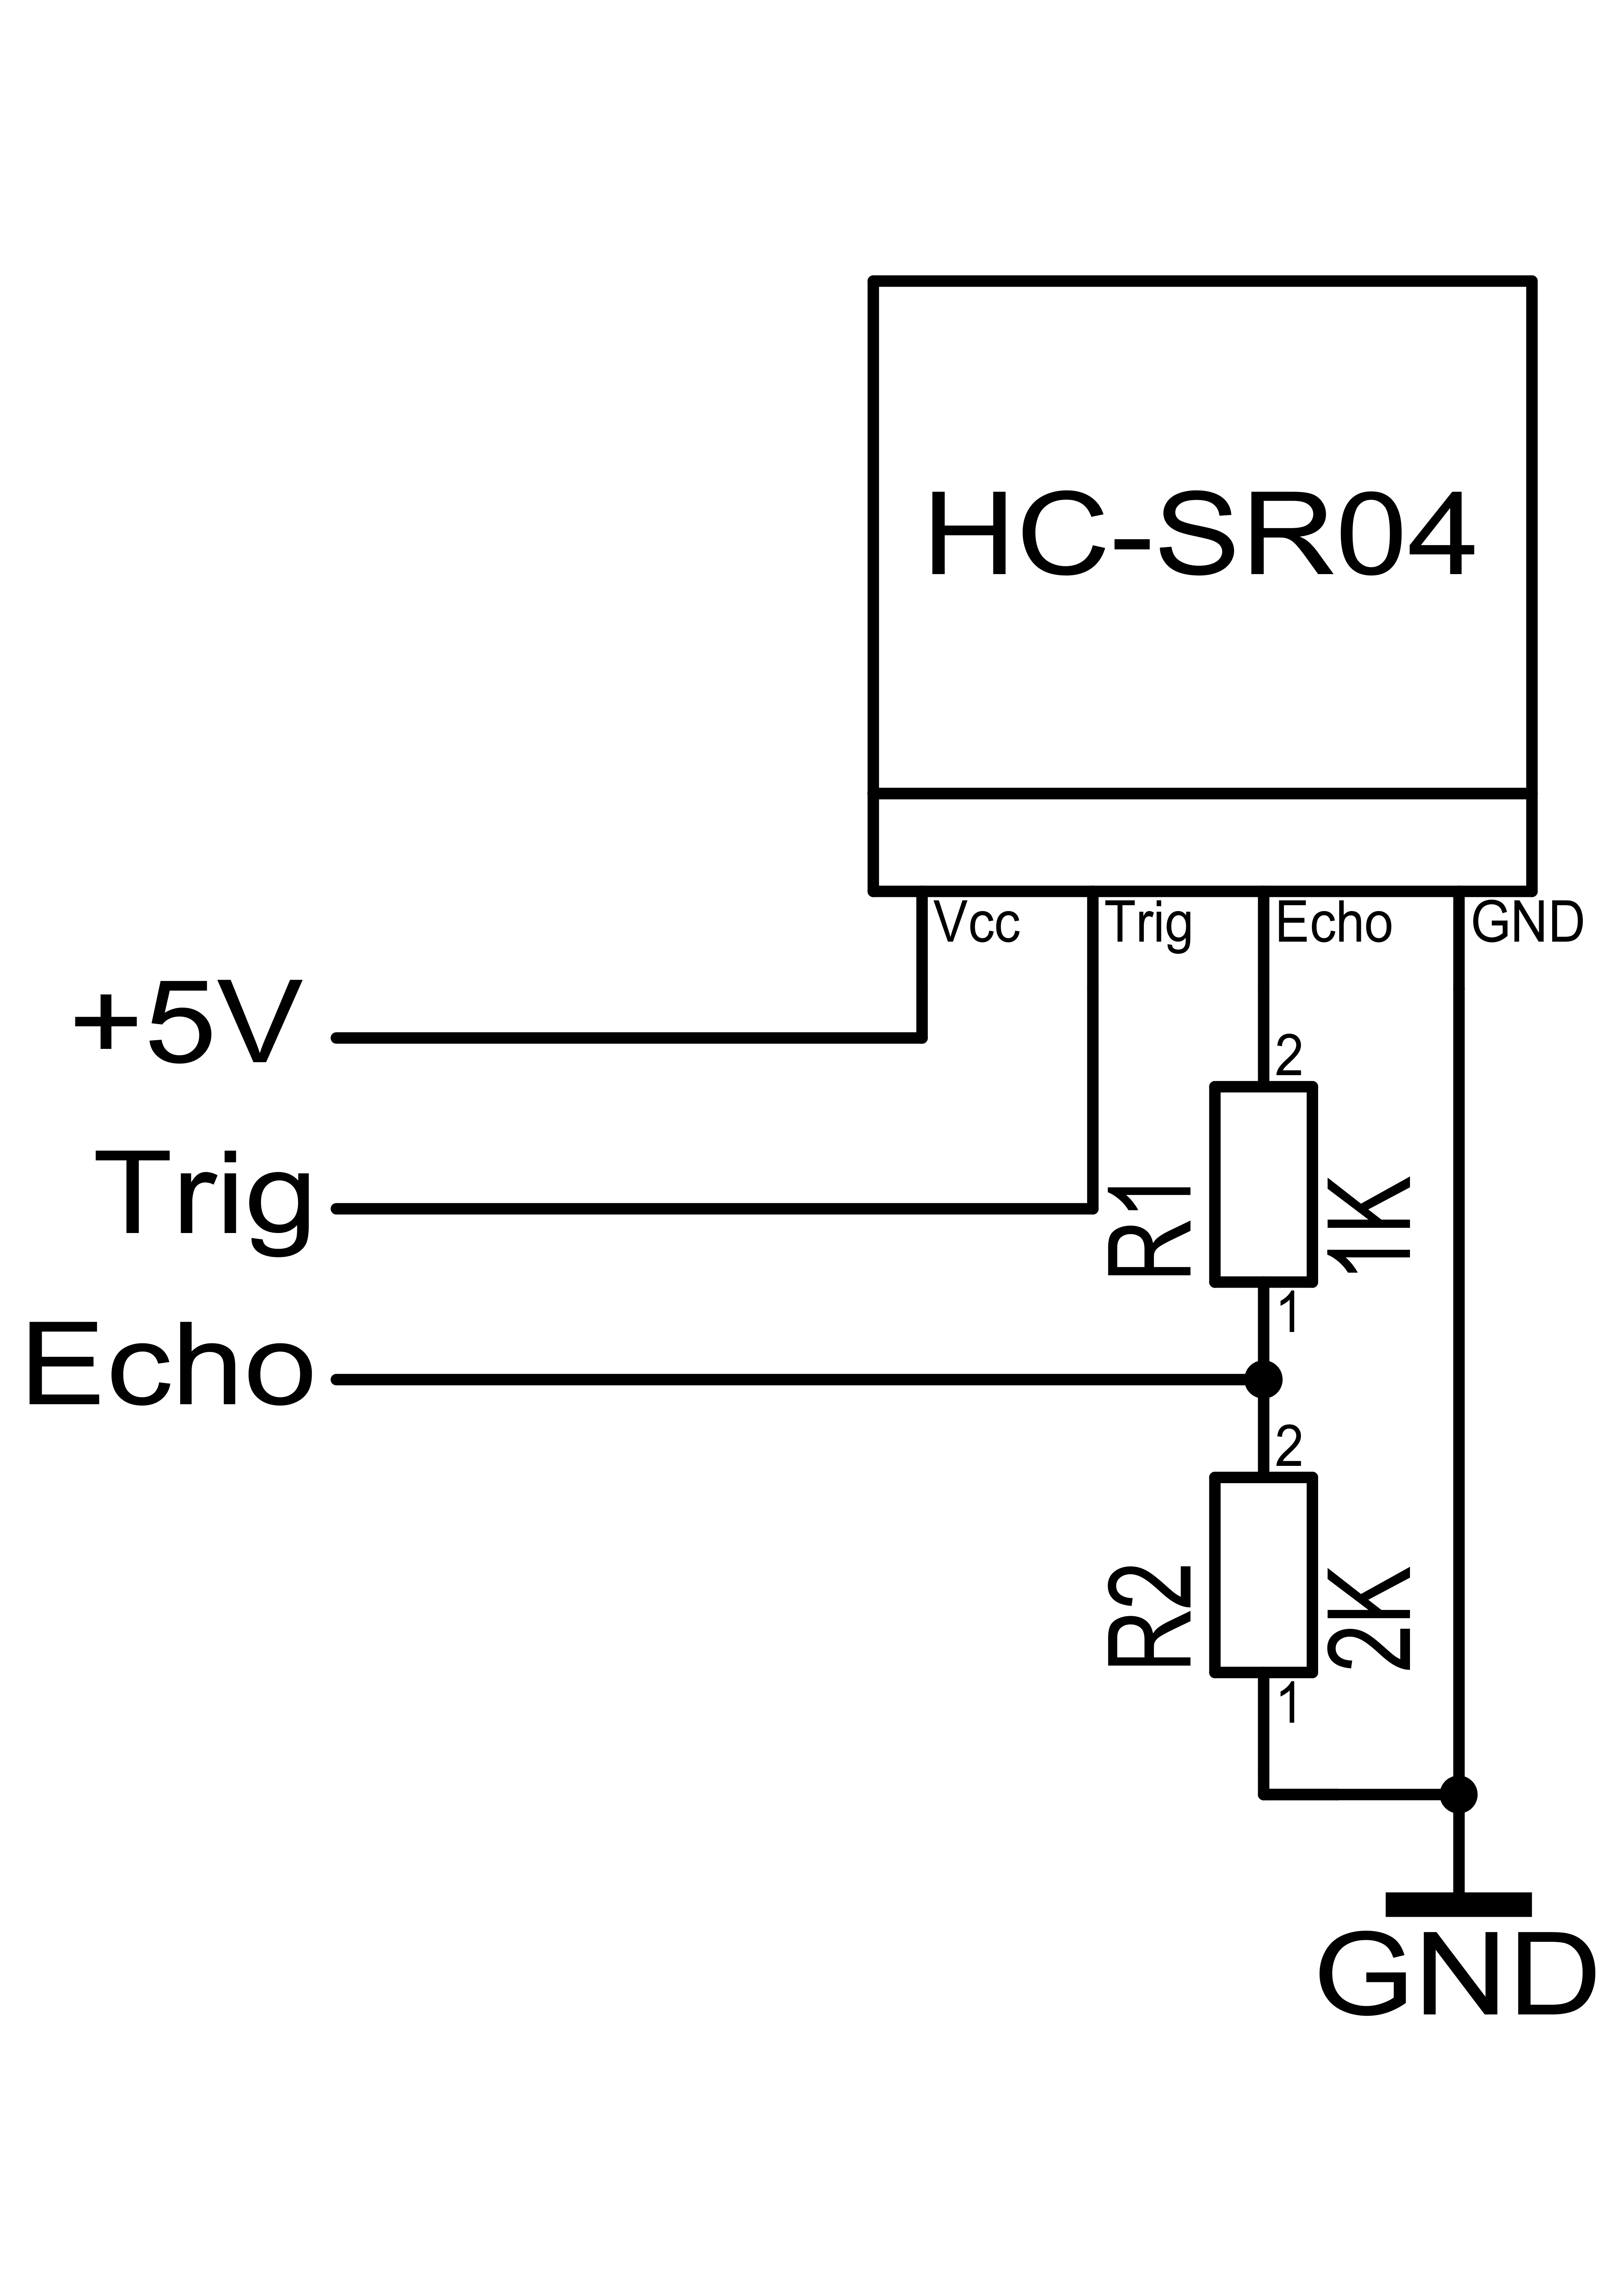
\includegraphics[scale=0.3]{immagini/HC-SR04_Circuito.png}
\caption{Circuito di interfaccia tra Arduino DUE e il sensore HC-SR04} 
\end{figure}

\section{Software}
\subsection {OpenCV}
\subsection {ADK}
In Android, a partire dalla versione 3.1, è supportato il protocollo Android Open 
Accessory (AOA), 
ogni accessorio sviluppato per Android deve supportare lo stesso protocollo. 
\\A causa della limitata autonomia dei dispositivi su cui Android è maggiormente 
utilizzato (smarthphone e tablet) l'AOA impone che l'accessorio funga da host 
e alimenti quindi il bus utlizzato
\\Per usare Arduino come un accessorio per Android e rispettare lo standard AOA 
esiste la libreria \textit{adk.h} che permette di dialogare con un dispositivo 
Android dopo un'accurata configurazione. Android distingue diversi accessori 
sulla base di informazioni che ogni accessorio fornisce all'atto della connessione, 
queste informazioni sono:
\begin{itemize}
\item Vendor
\item Name
\item Longname
\item Version
\item Url
\item Serial
\end{itemize} 
Il dispositivo Android accetterà la richiesta di connessione solo se le stringhe 
identificative in suo possesso combaciano perfettamente con quelle fornite 
dall'accessorio. Per ottenere effettivamente la connessione bisogna indicare ad 
Android quali sono gli accessori supportati e quale applicazioni è in grado di 
gestire un particolare accessorio. Questo si ottiene inserendo la successiva 
direttiva nel Manifest file dell'App

\lstset{language=XML}

\begin{lstlisting}[caption=Porzione del Manifest file dell'App]
...
<meta-data
    android:name="android.hardware.usb.action.
    				USB_ACCESSORY_ATTACHED"
    android:resource="@xml/usb_accessory_filter" />
...
\end{lstlisting}
In questo modo alla connessione di qualsiasi accessorio sarà il sistema operativo
a suggerire di aprire una certa app se l'accessorio connesso è presente nel file 
usb\_accessory\_filter.xml associato.
\\Nel nostro caso il file usb\_accessory\_filter.xml si presenta così
\begin{lstlisting}[caption=usb\_accessory\_filter.xml]
<resources>
    <usb-accessory
            version="0.1.0"
            model="Mobile-Tanker"
            manufacturer="Simone Mariotti"/>
</resources>
\end{lstlisting}
Le stesse identiche stringhe saranno impostate durante la fase di configurazione 
di Arduino in modo da permette l'accoppiamento.
\subsection {ADK Toolkit}
L'ADK toolkit è una libreria che aggiunge un grado di astrazione all'ADK, l'invio
 e la ricezione dei messaggi sono semplificati così come l'inizializzazione della 
 connessione.\\
Il toolkit si basa su due classi principali: AdkManager e AdkMessage.	\\	
AdkManager espone metodi per la gestione della connessione e per l'invio e la 
ricezioni di dati. AdkMessage rappresenta il messaggio ricevuto dall'accessorio 
ne suo formato nativo, cioè un array di byte; tramite dei metodi ausiliari, 
\textit{getString()}, \textit{getFloat()}, \textit{getInt()}, è possibile 
ottenere una versione tipizzata del messaggio e naturalmente la versione ``grezza'' 
dei dati con \textit{getBytes()} e \textit{getByte()}.\\
Grazie a questa libreria l'uso dell'ADK, originariamente poco intuitivo, diventa 
efficiente ed elegante
\lstset{
language=Java,
frame=tb,  
  aboveskip=3mm,
  belowskip=3mm,
  showstringspaces=false,
  columns=flexible,
  basicstyle={\small\ttfamily},
  numbers=none,
  identifierstyle=\color{black},
  numberstyle=\tiny\color{gray},
  keywordstyle=\color{blue},
  commentstyle=\color{dkgreen},
  stringstyle=\color{mauve},
  breaklines=true,
  breakatwhitespace=true,
  tabsize=3
}
\begin{lstlisting}[caption=Inizializzazione della connessione con l'accessorio]
private AdkManager mAdkManager;

@Override
protected void onCreate(Bundle savedInstanceState) {
    // ...
    mAdkManager = new AdkManager(this);
}

@Override
protected void onResume() {
    super.onResume();
    mAdkManager.open();
}
\end{lstlisting}
\begin{lstlisting}[caption=Lettura e scrittura dati]
// Write
adkManager.write("Ciao da Android!");

// Read
AdkMessage response = adkManager.read();
System.out.println(response.getString());
// Could outputs: "Ciao da Arduino!"
\end{lstlisting}